% !TEX root = ../main.tex
\documentclass[../main.tex]{subfiles}
\begin{document}
\subsection{Програмное обеспечение для компьютера: графический интерфейс}
Графический интерфейс программы представляет собой виджет PyQt5, он наследуется от класса \texttt{PyQt5.QtWidgets.QWidget}. Класс содержит следующие методы:

\begin{itemize}
    \item \texttt{\_\_init\_\_}
    \item \texttt{init\_ui}
    \item \texttt{autorange}
    \item \texttt{pressure\_diff}
    \item \texttt{init\_mic}
    \item \texttt{init\_bmp}
    \item \texttt{bmp\_update}
    \item \texttt{mic\_update}
    \item \texttt{closeEvent}
\end{itemize}

В начале класса объявляются статические поля - стандартный для PyQt5 способ обзявления сигналов:
\begin{lstlisting}
bmp_signal = PyQt5.QtCore.pyqtSignal()
mic_signal = PyQt5.QtCore.pyqtSignal()
\end{lstlisting}

\subsubsection{подключение сигналов к потоку сбора данных с USB}

В инициализаторе класса \texttt{\_\_init\_\_} эти сигналы подключаются к Qt-слотам: при срабатывании первого сигнала будет вызываться метод обновления графика датчкиков давления. А при срабатывании второго синнала будет вызываться метод обновления графика с микрофона а также графика FFT-спектра.

\begin{lstlisting}
def __init__(self):
    super().__init__()

    self.init_ui()

    self.bmp_signal.connect(self.bmp_update)
    self.mic_signal.connect(self.mic_update)
\end{lstlisting}

Также в инициализаторе класса при помощи ключевого слова super вызывается инициализатор родительского класса виджета. Далее вызывается метод \verb|init_ui| который создаст необходимые элементы интерфейса.

\subsubsection{инициализация графического интерфейса}
В данном методе иницализируются элементы графического интерфейса. Создается элемент \verb|layout = PyQt5.QtWidgets.QVBoxLayout()| - этот элемент позволяет добавлять в него другие элементы и распоолагать их вертикально. В этот \verb|layout| будут помещаться графики с датчиков давления, с микрофона и также график FFT для сигнала с микрофона. Также добавляется другой layout для кнопок управления.

С помощью вызова метода \verb|self.setGeometry(100, 100, 1200, 800)| задаются размеры окна-виджета приложения. Затем вызываются методы \texttt{init\_mic} и \verb|init_bmp|.

\subsubsection{инициализация графиков сигнала с микрофона}
В данном методе иницализируются параметры связанные с графиками сигнала с микрофона и графиком FFT. Объявляется буффер, в котором будут храниться значения с микрофона: 

\begin{lstlisting}
self.mic = np.full(self.mic_n, np.nan)
\end{lstlisting}

Указатель на текущее положение в буффере задается переменной \verb|mic_cursor|.

Создается объект fft графика:
\begin{lstlisting}
self.fft_plot = pyqtgraph.PlotWidget(disableAutoRange=True)
\end{lstlisting}

Графику добавляется сетка и включается логарифмический режим для осей X (частота звука) и Y (громкость звука в децибеллах):

\begin{lstlisting}
self.fft_plot.showGrid(x=True, y=True, alpha=0.15)
self.fft_plot.setLogMode(x=True, y=True)
\end{lstlisting}

Оба графика для сигнала и для фурье-образа добавляются на layout созданный в методе \verb|init_ui|:

\begin{lstlisting}
self.layout.addWidget(self.fft_plot)
self.layout.addWidget(self.mic_plot)
\end{lstlisting}


\subsubsection{инициализация графиков сигнала с датчиков давленя}
В данном методе инициализируются 2 буффера для хранения последних \texttt{self.bmp\_n = 100} показаний с датчиков давления:

\begin{lstlisting}
self.bmp0 = np.full(self.bmp_n, np.nan)
self.bmp1 = np.full(self.bmp_n, np.nan)
\end{lstlisting}

Изначально буфферы инициализируются значениями \verb|np.nan|. Это позволит не отображать их на графике и не сбивать масштаб по вертикали. \texttt{self.state = 'норм'}: иницализируется состояние (вдох/выдох/норм).

Определение вдоха или выдоха будет определяться на основе разнице с датчиков давления. Изначально в нормальном состояниии между датчиками тоже может присутсвовать разница. Поэтому нужно будет делать поправку на разность давления в нормальном состоянии (не вдох и не выдох). Это значение будет храниться в переменной \verb|self.normal_dp|.

\subsubsection{обновление графиков датчиков давления}
Данный метод вызывается по сигналу из потока \verb|serial_port| когда приходят новые данные с датчиков давления. В данном методе читаются данные из буфферов потока \verb|serial_port|. Полученные данные сохраняются в собственные буфферы  в классе \verb|GUI|: \verb|self.bmp0|, \verb|self.bmp0|.

С помощью новых данных обновляются кривие на графике:
\begin{lstlisting}
self.bmp0_curve.setData(self.bmp0)
self.bmp1_curve.setData(self.bmp1)
\end{lstlisting}

Если буфферы заполнились то они заполняются значениями \verb|np.nan|:

\begin{lstlisting}
if self.bmp_cursor == self.bmp_n:
    self.bmp0[:] = np.nan
    self.bmp1[:] = np.nan
    self.bmp_cursor = 0
\end{lstlisting}

Также в заголовок графика выводится состояние (вдох/выдох/норм):
\begin{lstlisting}
self.bmp_plot.setTitle(f'<h1>{state}  bmp0 - bmp1 = {bmp0 - bmp1:>+3.2f}</h1>')
\end{lstlisting}


\subsubsection{обновление графиков микрофона}
Данный метод обновляет график сигнала с микрофона и график FFT. Этот метод также вызывается по сигналу из процесса отвечающего за сбор данных с USB-устройства. После того как новые данные получены. То обновляются кривые на графиках:

\begin{lstlisting}
self.mic_curve.setData(self.mic)
self.fft_curve.setData(fft_f, fft_a)
\end{lstlisting}

В заголовок графика выводится частота дискретизации с которой был принят сигнал. (она может меняться со временем)
\begin{lstlisting}
self.mic_plot.setTitle(f'<h1>Sample Rate: {rate/1000:0.2f} kHz</h1>')
\end{lstlisting}

\subsubsection{обработка безопасного закрытия приложения}
Данный метод является стандартным для Qt методом который вызывается при закрытии приложения. (Например через значек (x) в полоске меню). При закрытии приложения устанавливается флаг для потока \verb|serial_port|. Когда эта переменная примет значение False, то поток прекратит прием данных с устройства и безопасно закроет соединение через последовательный порт.

\begin{lstlisting}
def closeEvent(self, event):
    serial_port.stop_flag = True
\end{lstlisting}

Схема основных элементов программного обеспечения для компьютера Arduino представлена на рисунке 18.

\begin{figure}[H]
\centering
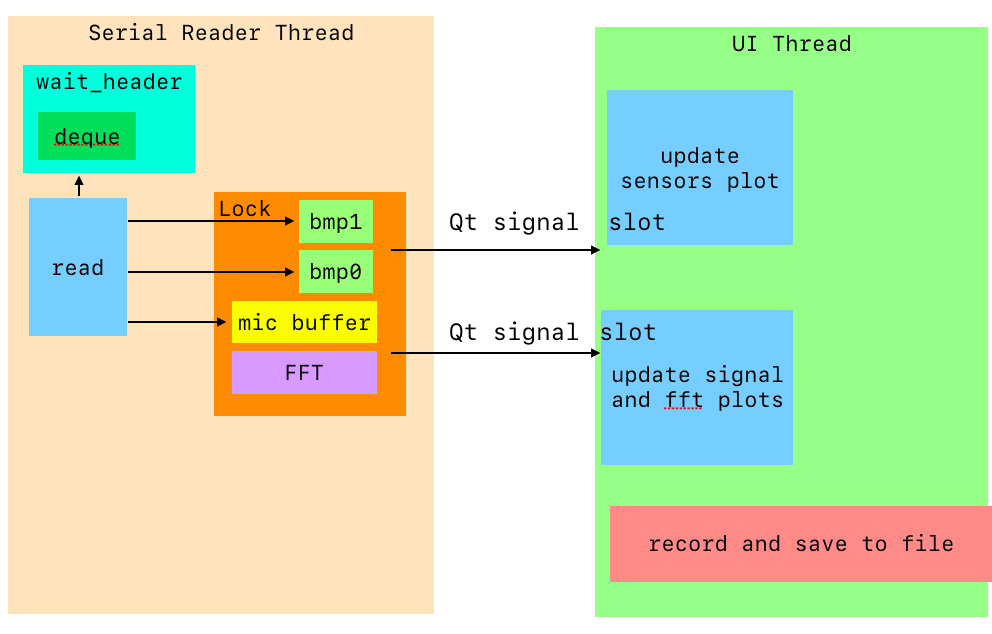
\includegraphics[width=\textwidth]{images/laptop-schema.png}
\caption{Диаграмма классов ПО для компьютера}
\end{figure}


\newpage
\end{document}
